\subsection{Probabilistic Trust}%
\label{sub:probabilistic_trust}
In our approach to a randomness beacon, we want to push beyond the need for honest operators, and naïve users.
To achieve this, we first need to quantify trusting the beacon and then determine thresholds for reasonable behaviour.
This effectively will provide a measure of probabilistic trust, where users much decide for themselves, if the probability of honest operation is adequate.

We present a property which, if satisfied, says that the user can trust that the beacon operator is not capable of fooling them.
The property is true if the user determines that nobody will be able to compute the delay function in the time between they sent their input and received the commitment.
This can be condensed to:
\begin{equation*}
    t_\text{COMMITMENT} - t_\text{INPUT} < T_\text{DELAY FUNCTION}
\end{equation*}
given that $t_\text{INPUT}$ is the time when the user sent the input, $t_\text{COMMITMENT}$ is when the user received the commitment, and $T_\text{DELAY FUNCTION}$ is the fastest computation of the delay function.
This tells us that for users to be more likely to trust a beacon, the time between them sending their input and receiving the commitment, must be significantly smaller than the time between the commitment and the output.
In fact, it must be smaller than the shortest time a given user thinks the operator could be able to compute the delay function.

Taking this into consideration we present a beacon operation protocol, which can be adjusted to increase or decrease this limit.
The operation must be sequential, which means that we must collect input before computing the delay function.
However, because we want to spend more time computing, than we are collecting input, a strictly sequential beacon will contain dead spots, where no user is submitting input.
This may be acceptable in some scenarios, but we want to design a beacon which always accepts inputs, and which will not be suspected of malicious operation.
To achieve this we parallelize the beacon protocol, meaning that several delay functions will run in parallel but offset in time, and using different input.

In~\cref{fig:beacon_parallel_timeline} this is illustrated, where these offset but parallel beacons are seen.
We observe that no input collection is run in parallel nor overlapping, which resembles a constant stream of input collection.
Moreover, the computation components can eventually be reused for future beacon computations, thereby eliminating the need for spinning up new computation services.
These observations are depicted in~\cref{fig:beacon_parallel_timeline_real}, where the beacon would output at each circle shown in the diagram.

\begin{figure}
    \centering
    \footnotesize
    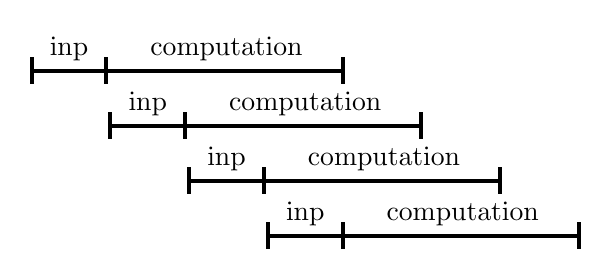
\begin{tikzpicture}
    \foreach \x in {0, 1, 2,...,3} {
        \draw[|-|, black, line width=0.5mm] (\x,-\x*0.7) to (\x+1,-\x*0.7);
        \path (\x,-\x*0.7) -- (\x+1,-\x*0.7) node [midway, above] {inp};
        \draw[-|, black, line width=0.5mm, shorten <=-0.1mm] (\x+1,-\x*0.7) to (\x+4,-\x*0.7);
        \path (\x+1,-\x*0.7) -- (\x+4,-\x*0.7) node [midway, above] {computation};
    }
    \end{tikzpicture}
    \caption{Parallelized beacon protocol, with offset input collection and overlapping computation.}\label{fig:beacon_parallel_timeline}
\end{figure}

\begin{figure}
    \centering
    \footnotesize
    \begin{tikzpicture}[xscale=0.95,
        comp line/.style={-o, GoogleIndigo, line width=0.5mm, shorten <=-0.1mm},
        incomplete comp line/.style={comp line, -ss},
        input line/.style={latex reversed-, dotted, black, line width=0.2mm},
    ]
    \pgfdeclarelayer{background}
    \pgfsetlayers{background,main}
    \draw[|-ss, line width=0.5mm, black] (0,0.7) to (8.5,0.7);
    \path (0,0.7) -- (8,0.7) node [midway, above] {Input Collection Stream};

    \foreach \x in {0, 1, 2} {
        \begin{pgfonlayer}{background}
            \draw[input line] (\x+1,0.7) to (\x+1,-\x*0.7);
        \end{pgfonlayer}
        \draw[comp line] (\x+1,-\x*0.7) to (\x+4,-\x*0.7);
        \path (\x+1,-\x*0.7) -- (\x+4,-\x*0.7) node [midway, above] {\contour{white}{Computation}};
    }
    \foreach \x in {3, 4} {
        \begin{pgfonlayer}{background}
        \draw[input line] (\x+1,0.7) to (\x+1,{-(\x-3)*0.7});
        \end{pgfonlayer}
        \draw[comp line] (\x+1,{-(\x-3)*0.7}) to (\x+4,{-(\x-3)*0.7});
        \path (\x+1,{-(\x-3)*0.7}) -- (\x+4,{-(\x-3)*0.7}) node [midway, above] {\contour{white}{Computation}};
    }

    \begin{pgfonlayer}{background}
    \draw[input line] (6,0.7) to (6,-0.7*2);
    \end{pgfonlayer}
    \draw[incomplete comp line] (6,-0.7*2) to (8.5,-0.7*2);
    \path (6+1.5,-0.7*2) node [above] {\contour{white}{Computation}};

    \begin{pgfonlayer}{background}
    \draw[input line] (7,0.7) to (7,0);
    \end{pgfonlayer}
    \draw[incomplete comp line] (7,0) to (8.5,0);

    \begin{pgfonlayer}{background}
    \draw[input line] (8,0.7) to (8,-0.7);
    \end{pgfonlayer}
    \draw[incomplete comp line] (8,-0.7) to (8.5,-0.7);

    \end{tikzpicture}
    \caption{Parallelized beacon protocol, with input collection stream and overlapping computation. A circle denotes outputting at the end of the computation.}\label{fig:beacon_parallel_timeline_real}
\end{figure}
